% Template file for an a0 landscape poster.
% Written by Graeme, 2001-03 based on Norman's original microlensing
% poster.
%
% See discussion and documentation at
% <http://www.astro.gla.ac.uk/users/norman/docs/posters/> 
%
% $Id: poster-template-landscape.tex,v 1.2 2002/12/03 11:25:46 norman Exp $


% Default mode is landscape, which is what we want, however dvips and
% a0poster do not quite do the right thing, so we end up with text in
% landscape style (wide and short) down a portrait page (narrow and
% long). Printing this onto the a0 printer chops the right hand edge.
% However, 'psnup' can save the day, reorienting the text so that the
% poster prints lengthways down an a0 portrait bounding box.
%
% 'psnup -w85cm -h119cm -f poster_from_dvips.ps poster_in_landscape.ps'

\documentclass[a0]{a0poster}
% You might find the 'draft' option to a0 poster useful if you have
% lots of graphics, because they can take some time to process and
% display. (\documentclass[a0,draft]{a0poster})
\input defs
\pagestyle{empty}
\setcounter{secnumdepth}{0}
\renewcommand{\familydefault}{\sfdefault}
\newcommand{\QED}{~~\rule[-1pt]{8pt}{8pt}}\def\qed{\QED}

\renewcommand{\reals}{{\mbox{\bf R}}}

% The textpos package is necessary to position textblocks at arbitary 
% places on the page.
\usepackage[absolute]{textpos}

\usepackage{fleqn,psfrag,wrapfig,tikz,amsmath, framed, scrextend,subcaption}
\usepackage{mathtools,url}
\DeclarePairedDelimiterX{\norm}[1]{\lVert}{\rVert}{#1}

\usepackage[papersize={38in,28in}]{geometry}

% Graphics to include graphics. Times is nice on posters, but you
% might want to switch it off and go for CMR fonts.
\usepackage{graphics}

\renewenvironment{leftbar}[1][\hsize]
{% 
\def\FrameCommand 
{%

    {\color{black}\vrule width 0pt}%
    \hspace{0pt}%must no space.
    \fboxsep=\FrameSep\colorbox{white}%
}%
\MakeFramed{\hsize#1\advance\hsize-\width\FrameRestore}%
}
{\endMakeFramed}

% we are running pdflatex, so convert .eps files to .pdf
%\usepackage[pdftex]{graphicx}
%\usepackage{epstopdf}

% These colours are tried and tested for titles and headers. Don't
% over use color!
\usepackage{color}
\definecolor{Red}{rgb}{0.9,0.0,0.1}

\definecolor{bluegray}{rgb}{0.15,0.20,0.40}
\definecolor{bluegraylight}{rgb}{0.35,0.40,0.60}
\definecolor{gray}{rgb}{0.3,0.3,0.3}
\definecolor{lightgray}{rgb}{0.7,0.7,0.7}
\definecolor{darkblue}{rgb}{0.2,0.2,1.0}
\definecolor{darkgreen}{rgb}{0.0,0.5,0.3}

\renewcommand{\labelitemi}{\textcolor{bluegray}\textbullet}
\renewcommand{\labelitemii}{\textcolor{bluegray}{--}}

\setlength{\labelsep}{0.5em}


% see documentation for a0poster class for the size options here
\let\Textsize\normalsize
%\def\Head#1{\noindent\hbox to \hsize{\hfil{\LARGE\color{bluegray} #1}}\bigskip}
\def\Head#1{\noindent{\LARGE\color{bluegray} #1}\bigskip}
\def\LHead#1{\noindent{\LARGE\color{bluegray} #1}\bigskip}
\def\Subhead#1{\noindent{\large\color{bluegray} #1}\bigskip}
\def\Title#1{\noindent{\VeryHuge\color{Red} #1}}

\usepackage{multicol}
\setlength{\columnsep}{1cm}

% Set up the grid
%
% Note that [40mm,40mm] is the margin round the edge of the page --
% it is _not_ the grid size. That is always defined as 
% PAGE_WIDTH/HGRID and PAGE_HEIGHT/VGRID. In this case we use
% 23 x 12. This gives us three columns of width 7 boxes, with a gap of
% width 1 in between them. 12 vertical boxes is a good number to work
% with.
%
% Note however that texblocks can be positioned fractionally as well,
% so really any convenient grid size can be used.
%
\TPGrid[40mm,40mm]{23}{12}      % 3 cols of width 7, plus 2 gaps width 1

\parindent=0pt
\parskip=0.2\baselineskip

\begin{document}

% Understanding textblocks is the key to being able to do a poster in
% LaTeX. In
%
%    \begin{textblock}{wid}(x,y)
%    ...
%    \end{textblock}
%
% the first argument gives the block width in units of the grid
% cells specified above in \TPGrid; the second gives the (x,y)
% position on the grid, with the y axis pointing down.

% You will have to do a lot of previewing to get everything in the 
% right place.

% This gives good title positioning for a portrait poster.
% Watch out for hyphenation in titles - LaTeX will do it
% but it looks awful.
\begin{textblock}{23}(0,0)
\Title{Diabetes Prediction with Incomplete Patient Data}
\end{textblock}

\begin{textblock}{23}(0,0.6)
{
\LARGE
Hao Yi Ong,
Dennis Wang,
Xiao Song Mu
}

{
\Large
\color{bluegray}
\emph{CS 221 Artificial Intelligence: Principles and Techniques Class Project}
}
\end{textblock}


% Uni logo in the top right corner. A&A in the bottom left. Gives a
% good visual balance, but you may want to change this depending upon
% the graphics that are in your poster.
%\begin{textblock}{2}(0,10)
%Your logo here
%%\includegraphics{/usr/local/share/images/AandA.epsf}
%\end{textblock}

% \begin{textblock}{3}(21.0,0)
% % Another logo here
% \resizebox{1.95\TPHorizModule}{!}{
\includegraphics{uni-logo.png}}
% \end{textblock}


\begin{textblock}{7.0}(0,1.5)

\hrule\medskip
\Head{Introduction}

\begin{itemize}
  
  \item Given a set of electronic health records, we want to have a smart predictor that prompts high-risk patients to obtain Type II Diabetes testing

\end{itemize}

\begin{figure}[!h]
  \centering
  
\includegraphics[width=9in]{intro-fig.pdf}
  \label{fig1}
\end{figure}

\begin{multicols}{2}
  
  \begin{itemize}
    \item Original Kaggle challenge:
    \begin{itemize}
      \item Patients all have a standard database and a full medical record
      \item I.e., exact same tests taken, same variables recorded, etc.
    \end{itemize}

    \item In practice, however:
    \begin{itemize}
      \item Not everyone has taken the same tests and gotten regular checkups
      \item Database inconsistencies or errors in inputting data may exist
    \end{itemize}
  \end{itemize}
\end{multicols}

\begin{itemize}

  \item Predictor must be able to accurately classify based on incomplete or erroneous medical records to be useful

\end{itemize}

\medskip
\hrule\medskip
\Head{Diabetes Prediction}

\begin{itemize}

  \item Given
  \begin{itemize}
    \item \emph{Training set} containing standardized patient medical records
    \item \emph{Testing set} containing patient medical records with missing information and unknown erroneously recorded data
  \end{itemize}

  \item Output
  \begin{itemize}
    \item \emph{Bayesian network structure} encoding the conditional dependencies between medical record variables
    \item \emph{Bayesian network parameters} encoding the conditional probabilities for each variable
    \item \emph{Probabilistic inference} on the learned Bayesian network (BN) for classification
  \end{itemize}

  \item To minimize the error rate, including false positives and false negatives, on classifying whether a patient has Type II Diabetes

\end{itemize}

\medskip
\hrule\medskip
\Head{Evaluation Criteria}

\begin{figure}[!h]
  \centering
  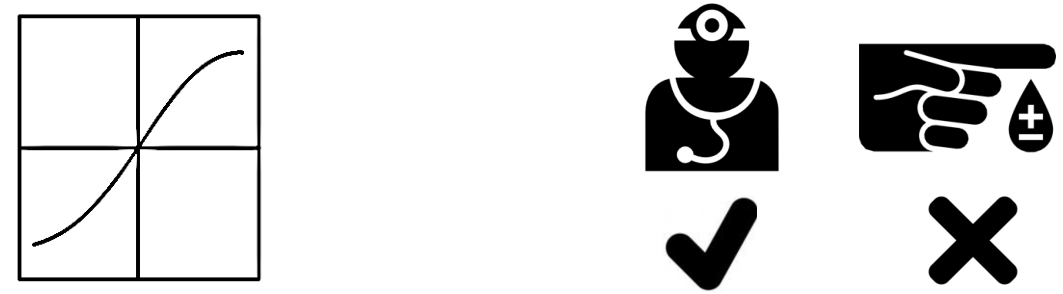
\includegraphics[width=0.8\textwidth]{eval-fig.pdf}
  \label{fig2}
\end{figure}

\begin{multicols}{2}
  \begin{itemize}
    
    \item \emph{Baseline} of logistic regression
    \begin{itemize}
      \item Basic features: age, BMI, ...
      \item 10\% hold-out cross validation
      \item False positive rate of 0.7\%, false negative rate of 15.3\%, and an error rate of 16\% (84\% accuracy)
    \end{itemize}

    \item \emph{Oracle}
    \begin{itemize}
      \item Ideal oracle: experienced physicians (impractical)
      \item Use as surrogate diabetes tests vetted by HHS (HBA1c, FPG, and OGTT; 85--95\% accuracy)
    \end{itemize}

  \end{itemize}
\end{multicols}

\end{textblock}

\begin{textblock}{7.0}(8,1.5)

\hrule\medskip
\Head{Structure Learning as a Search Problem}\vspace{-1em}

\begin{itemize}
  
  \item \textbf{NP-hard search problem} Finding the best set of edges is hard as the number of BNs (DAGs) grows superexponentially with the number of nodes

  \item \textbf{Bayesian score} To evaluate the BN, we use the Bayesian score, which optimally balances the complexity of the BN structure with the available data (Koller and Friedman, 2009)

  \item \textbf{Feature selection} We manually selected 27 discretized features (nodes) according to ICD9 disease groupings to limit the search space

  \item \textbf{Tabu search} To find the optimal structure, we use a hill-climbing algorithm that maximizes the ``fitness'' of the BN based on the Bayesian score

  By maintaining a tabu list of recent operators we applied (e.g., adding an edge to the existing BN) and not considering operators that reverse the effect of recently applied operators, the heuristic avoids getting stuck at local optima

  \medskip \hrule
  \begin{addmargin}[0em]{2em}% 5em left, 2em right
    \begin{leftbar}
      \begin{tabbing}
        {\bf given} training set \(\mathcal{D}\), structure prior \(P(\mathcal{G})\), node set \(\mathcal{N}\), tabu list size \(L\) \\*[\smallskipamount]
        {\bf initialize} random BN \(\mathcal{G}\), tabu list \(\mathcal{T}\), valid operations \(\mathcal{O}\) \\*[\smallskipamount]
        {\bf repeat} \\
        \qquad \= 1.\ if \(\left|\mathcal{O}\right|\) too large, generate random subset of valid operations \(\hat{\mathcal{O}}\subset\mathcal{O}\) \\
        \> 2.\ find best operation: \(\text{Op} := \argmax_{\text{Op}\in\hat{\mathcal{O}}\backslash \mathcal{T}}\text{BayesScore}(\text{Op}(\mathcal{G}))\) \\
        \> 3.\ set \(\mathcal{G}:=\text{Op}(\mathcal{G})\) and \(\mathcal{T}:=\mathcal{T}\cup\left\{\text{reverse}(\text{Op})\right\}\) \\
        \> 4.\ remove operation added \(L\) iterations ago to \(\mathcal{T}\) from it \\
        {\bf until} \(\text{BayesScore}(\mathcal{G})\) converges \\*[\smallskipamount]
        {\bf return} \(\mathcal{G}\)
      \end{tabbing}
    \end{leftbar}
  \end{addmargin}
  \hrule

\end{itemize}

\end{textblock}

\begin{textblock}{7.0}(8,6.8)

\begin{itemize}

  \item \textbf{Resulting structure} Below is the best structure out of 20 trials with a uniform Dirichlet prior over network structures
  \begin{figure}[!h]
    \centering
    \hbox{
      \hspace{-4em}
      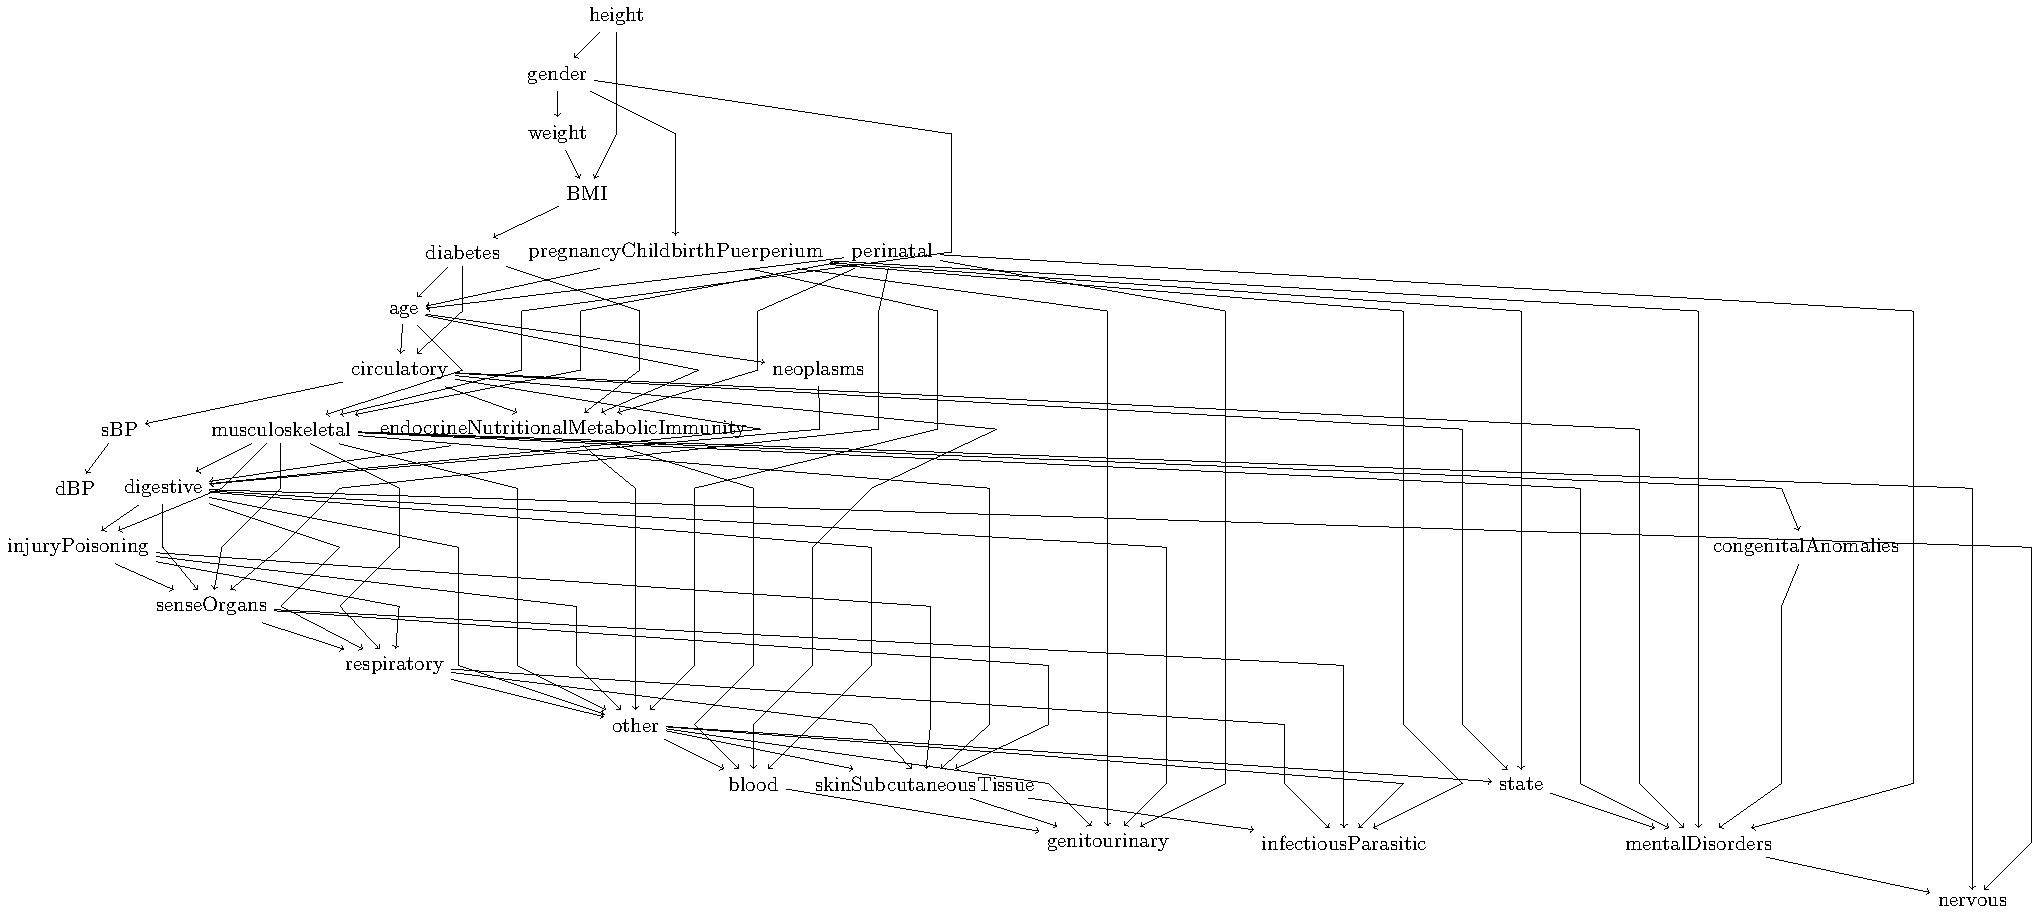
\includegraphics[width=1.2\textwidth]{bn-struct.pdf}
    }
    \label{fig3}
  \end{figure}

\end{itemize}

\end{textblock}

\begin{textblock}{7.0}(8,10.1)

\hrule\medskip
\Head{Parameter Learning}

\begin{itemize}

\end{itemize}
  
\end{textblock}
  
\begin{textblock}{7.0}(16,1.5)

\hrule\medskip
\Head{Approximate Probabilistic Inference}



\hrule\medskip
\Head{Conclusion}



\medskip

\hrule\medskip
\Head{Acknowledgments}

We thank Professor Liang and the instructor team, as well as fellow classmates for their help on our project.

\end{textblock}

\end{document}
